    \subsection*{Adding a second layer}
    
        So, let's add one more \textbf{layer}. We'll label layers by using a \textbf{superscript}: $W^1$ is the set of \textbf{weights} for the \textbf{first} layer, for example.
        
        \begin{figure}[H]
            \centering
            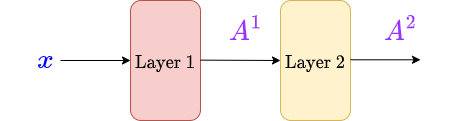
\includegraphics[width=100mm,scale=0.4]{images/nn_images/two_layers.png}
            \caption*{We have two separate outputs: $A^1$ and $A^2$.}
        \end{figure}
        
        \begin{clarification}
            \vocab{Superscripts} in our notation indicate the \purp{layer} that our value is associated with.
            
            They do \purp{not} represent exponentiation! 
        \end{clarification}
        
        \miniex $Z^3$ would be the \textbf{pre-activation} for layer 3: it is \textbf{not} Z "cubed".
        
        What can we learn from this?
        
        \begin{itemize}
            \item The \textbf{output} of layer 1, $A^1$, is the \textbf{input} to layer 2.
            
            \item Thus, the output dimension $n^1$ of layer 1 must \textbf{match} the input $m^2$ of layer 2: 
            
            \begin{equation}
                n^1=m^2
            \end{equation}
        \end{itemize}
        
        Let's break these into their components again.
        
        \begin{figure}[H]
            \centering
            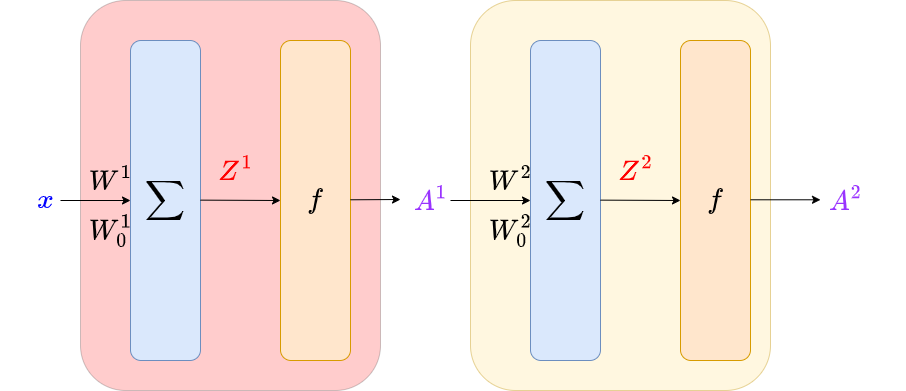
\includegraphics[width=100mm,scale=0.4]{images/nn_images/two_layers_internal.png}
            \caption*{We have two separate outputs: $A^1$ and $A^2$.}
        \end{figure}
        
        To distinguish between the linear functions in each layer, we'll just notate them using the weights and offsets.
        
        \begin{figure}[H]
            \centering
            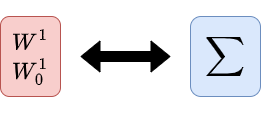
\includegraphics[width=40mm,scale=0.4]{images/nn_images/linear_module_representation.png}
            \caption*{These two are equivalent (if in the same layer)! We'll use the notation on the left, so that you know which layer our unit is in.}
        \end{figure}
        
        And this gives us:
        
        \begin{figure}[H]
            \centering
            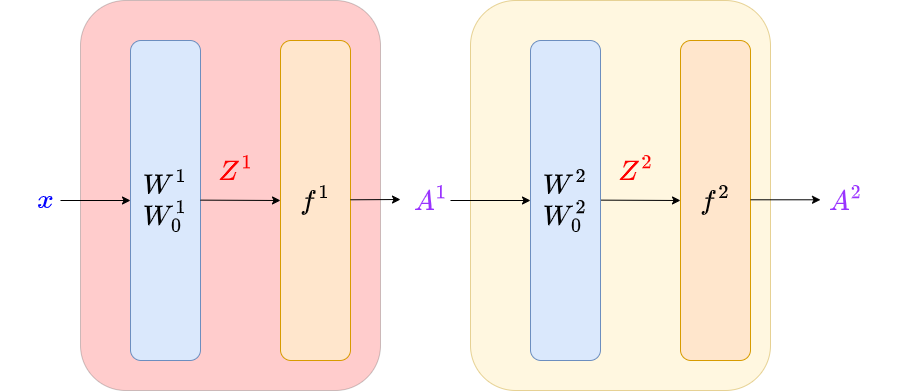
\includegraphics[width=100mm,scale=0.4]{images/nn_images/two_layer_new_notation.png}
        \end{figure}
        
        Now, we can make our functions. For layer one:
        
        \begin{equation}
            \red{A^1} = f(Z^1) = 
            f  
            \Big( 
                (\red{W^1})^T x + \red{W_0^1} 
            \Big)
        \end{equation}
        
        And layer two:
        
        \begin{equation}
            \blu{A^2} = f(Z^2) = 
            f  
            \Big( 
                (\blu{W^2})^T \red{A^1} + \blu{W_0^2} 
            \Big)
        \end{equation}
        
        We can use this to build our \textbf{general} pattern.
        